\documentclass[../main.tex]{subfiles}
\begin{document}
\section{程序测试}

% 给出测试报告,包括:
% 1)测试环境
% 2)测试的功能
% 3)针对每个功能的测试情况,包括:测试用例、预期的结果、测试结果及其分析
% 在设计测试计划时,不但要考虑正确的测试用例,还要考虑含有错误的测试用例

\subsection{测试环境}

本项目的测试分为单元测试、集成测试两个部分。其中,单元测试基于Xunit框架使用代码编写,集成测试则是将Pascal源文件分别使用\texttt{Free Pascal Compiler}编译器和自行实行的编译器之后运行之后对比输出。

\paragraph{本地测试环境}
\begin{itemize}
  \item \textbf{操作系统}: Arch Linux 6.8.9-zen1-2-zen (64-bit)
  \item \textbf{处理器}: 16 × 11th Gen Intel® Core™ i7-11800H @ 2.30GHz
  \item \textbf{内存}: 15.4 GiB of RAM
  \item \textbf{编译器}: Dotnet 8.0.104
  \item \textbf{开发环境}: JetBrains Rider
\end{itemize}

\paragraph{集成测试平台}
\begin{itemize}
  \item \textbf{操作系统}: Arch Linux 6.8.9-zen1-2-zen (64-bit)
  \item \textbf{处理器}: 16 × 11th Gen Intel® Core™ i7-11800H @ 2.30GHz
  \item \textbf{内存}: 15.4 GiB of RAM
  \item \textbf{C语言编译器}: GCC 14.1.1
  \item \textbf{Free Pascal Compiler编译器}: Free Pascal Compiler version 3.2.2
\end{itemize}

\subsection{单元测试}

单元测试需要对程序的一个或多个部分进行测试,因此不仅对本部分功能进行测试,还对与其他部分的协同工作进行测试。以下先介绍代码中各个目录涉及到的测试功能,再根据逻辑上的编译器划分进行逐部分功能说明。

\begin{itemize}
    \item \texttt{SemanticTests} 对字符(SemanticToken)的识别功能进行测试。
    \item \texttt{LexicalParserTests} 对词法分析器(Lexer)进行词法单元识别功能测试。
    \item \texttt{GrammarParserTests} 对语法分析器(GrammarParser)进行正确性和稳健性测试。
    \item \texttt{GeneratedParserTests} 对GeneratedGrammarParser能否正确生成语法解析进行测试。
\end{itemize}

\subsubsection{词法分析}

词法分析的功能为:将输入的Pascal程序按照一定规则以记号流的方式输出给后面的分析器,因此此处测试的主要任务应该是检查词法分析器能否正确识别程序中的"词语",并按照记号流的方式输出。因此我们通过对单一类型记号的测试,多种类型记号的混合测试,完整程序的验证测试来完成对词法分析的检查。

\begin{table}[H] % 使用 [H] 选项将表格固定在当前位置
\centering % 让表格内的文字居中
\caption{
\label{tab:test}词法分析功能说明} 
\begin{tabular}{c|p{10cm}} % 修改第一列为居中显示
\hline
\textbf{测试文件} & \textbf{功能} \\ 
\hline
CharacterTypeTests.cs & 测试对语句能否正确分隔,未定义符号能否识别报错 \\ 
DelimiterTests.cs & 对Delimiter分隔符的识别 \\ 
ErrorSingleTests.cs & 对字符串中的错误识别,以及非法字符的识别 \\ 
IndentifierTypeTests.cs & 标识符,与标识符类似的记号 \\
KeywordTypeTests.cs & 关键字识别 \\
LexicalFileTests.cs & 对词法分析器的总体功能测试,手动打表验证对pascal文件读取后的记号流输出。以及能否正确跳过注释 \\
NumberTests.cs & 对科学计数法、浮点数、十六进制等不同类型数字的识别 \\
OperatorTypeTests.cs & 对运算符的识别 \\
\hline
\end{tabular}
\end{table}

\paragraph{基础测试}
通过简单的输入,如数字序列和简单运算表达式,验证词法分析器是否能正确分辨和生成对应的标记。

\begin{itemize}
    \item \textbf{输入}:
    \begin{verbatim}
    123 + 456 - 789
    \end{verbatim}
    \item \textbf{预期输出}:
    \begin{itemize}
        \item 三个 \texttt{TOK\_INTEGER} 分别对应数值 123, 456, 789
        \item 一个 \texttt{TOK\_PLUS} 和一个 \texttt{TOK\_MINUS} 对应加号和减号
    \end{itemize}
\end{itemize}

\paragraph{注释} 
验证词法分析器是否能正确忽略Pascal代码中的单行和多行注释。

\begin{itemize}
    \item \textbf{输入}:
    \begin{verbatim}
    // This is a single line comment
    begin end.
    \end{verbatim}
    \item \textbf{预期输出}:
    \begin{itemize}
        \item 词法分析器应忽略注释,正确识别 \texttt{begin} 和 \texttt{end.} 标记
    \end{itemize}
\end{itemize}

\begin{itemize}
    \item \textbf{输入}:
    \begin{verbatim}
    {
        This is a
        multi-line comment
    }
    begin end.
    \end{verbatim}
    \item \textbf{预期输出}:
    \begin{itemize}
        \item 注释被正确忽略,仅识别 \texttt{begin} 和 \texttt{end.} 标记
    \end{itemize}
\end{itemize}

\paragraph{标识符和关键字}
验证词法分析器对Pascal关键字和用户定义的标识符的识别能力。

\begin{itemize}
    \item \textbf{输入}:
    \begin{verbatim}
    program test; var x: integer;
    \end{verbatim}
    \item \textbf{预期输出}:
    \begin{itemize}
        \item 关键字 \texttt{program}, \texttt{var}, \texttt{integer} 以及标识符 \texttt{test}, \texttt{x} 被正确识别
    \end{itemize}
\end{itemize}

\paragraph{字符串和字符识别}
测试词法分析器对字符串和字符字面量的处理。

\begin{itemize}
    \item \textbf{输入}:
    \begin{verbatim}
    'Hello, World!' "A"
    \end{verbatim}
    \item \textbf{预期输出}:
    \begin{itemize}
        \item 一个 \texttt{TOK\_STRING} 为 "Hello, World!"
        \item 一个 \texttt{TOK\_CHAR} 为 'A'
    \end{itemize}
\end{itemize}

\paragraph{CharacterTypeTests.cs}
此测试类用于验证字符和字符串类型的正确识别,确保词法分析器可以正确处理单个字符和字符串。

\textbf{测试方法:}使用ILexer接口的Tokenize方法处理输入的字符和字符串,然后检查生成的SemanticToken对象是否与预期的类型和值匹配。

\textbf{关键代码片段:}
\begin{lstlisting}[style=csharp]
[InlineData("'a'", 'a')]
[InlineData("'+'", '+')]
public void TestCharacterType(string input, char expectedResult)
{
    IEnumerable<SemanticToken> tokensEnumerable = _lexer.Tokenize(new StringSourceReader(input));
    List<SemanticToken> tokens = tokensEnumerable.ToList();
    Assert.Equal(SemanticTokenType.Character, tokens[0].TokenType);
    Assert.Equal(expectedResult, tokens[0].Convert<CharacterSemanticToken>().ParseAsCharacter());
}
\end{lstlisting}

通过上述测试,词法分析器能正确识别并返回字符类型的SemanticToken。

\paragraph{DelimiterTests.cs}

此测试类专注于分隔符的正确识别,包括逗号、冒号、分号等,验证它们是否被正确地解析为相应的DelimiterSemanticToken。

\textbf{测试方法:}对不同的分隔符进行词法分析,检查是否能正确地识别和返回相应的SemanticToken类型。

\textbf{关键代码片段:}
\begin{lstlisting}[style=csharp]
[InlineData(",123", DelimiterType.Comma)]
[InlineData(":123", DelimiterType.Colon)]
public void SmokeTest(string input, DelimiterType type)
{
    IEnumerable<SemanticToken> tokensEnumerable = _lexer.Tokenize(new StringSourceReader(input));
    List<SemanticToken> tokens = tokensEnumerable.ToList();
    SemanticToken token = tokens[0];
    Assert.Equal(SemanticTokenType.Delimiter, token.TokenType);
    DelimiterSemanticToken delimiterSemanticToken = (DelimiterSemanticToken)token;
    Assert.Equal(type, delimiterSemanticToken.DelimiterType);
}
\end{lstlisting}

此测试展示了词法分析器如何处理和识别各种分隔符,并将其准确分类为DelimiterSemanticToken。

\paragraph{ErrorSingleTests.cs}
此部分测试聚焦于词法分析器对不合法输入的处理,包括非法数字格式、未闭合的字符串、未知字符等错误。

\textbf{测试方法:}验证词法分析器在遇到错误输入时是否能正确抛出LexemeException,并准确标记错误发生的位置。

\textbf{关键代码片段:}
\begin{lstlisting}[style=csharp]
[InlineData("program main; var a: integer; begin a := 3#; end.", 1, 43, LexemeErrorType.IllegalNumberFormat)]
public void TestUnknownCharacterError(string pascalProgram, uint expectedLine, uint expectedCharPosition, LexemeErrorType expectedErrorType)
{
    var ex = Assert.Throws<LexemeException>(() => _lexer.Tokenize(new StringSourceReader(pascalProgram)).ToList());
    _testOutputHelper.WriteLine(ex.ToString());
    Assert.Equal(expectedErrorType, ex.ErrorType);
    Assert.Equal(expectedLine, ex.Line);
    Assert.Equal(expectedCharPosition, ex.CharPosition);
}
\end{lstlisting}
此测试检验了词法分析器在处理输入错误时的反应能力,包括正确抛出异常和提供错误发生的具体位置。


\paragraph{IdentifierTypeTests.cs}
此测试类用于检验标识符的正确识别,确保词法分析器能准确处理包含各种字符组合的标识符。

\textbf{测试方法:}通过ILexer接口的Tokenize方法处理不同样式的标识符输入,验证返回的SemanticToken是否正确标识为标识符类型。

\textbf{关键代码片段:}
\begin{lstlisting}[style=csharp]
[InlineData("identifier", true)]
[InlineData("_identifier", true)]
[InlineData("IdentifierWithCamelCase", true)]
public void TestParseIdentifier(string input, bool expectedResult)
{
    IEnumerable<SemanticToken> tokensEnumerable = _lexer.Tokenize(new StringSourceReader(input));
    List<SemanticToken> tokens = tokensEnumerable.ToList();
    Assert.Equal(expectedResult, tokens.FirstOrDefault()?.TokenType == SemanticTokenType.Identifier);
}
\end{lstlisting}
此测试确保了各种格式的标识符能被词法分析器正确识别。

\paragraph{KeywordTypeTests.cs}
此测试类用于验证关键字的正确识别,确保词法分析器可以正确区分和标识Pascal中的关键字。

\textbf{测试方法:}对一系列预定义的关键字进行解析,检查是否能被正确地标记为关键字类型的SemanticToken。

\textbf{关键代码片段:}
\begin{lstlisting}[style=csharp]
[InlineData("program", KeywordType.Program)]
[InlineData("var", KeywordType.Var)]
[InlineData("begin", KeywordType.Begin)]
public void SmokeTest(string input, KeywordType type)
{
    IEnumerable<SemanticToken> tokensEnumerable = _lexer.Tokenize(new StringSourceReader(input));
    List<SemanticToken> tokens = tokensEnumerable.ToList();
    SemanticToken token = tokens[0];
    Assert.Equal(SemanticTokenType.Keyword, token.TokenType);
    KeywordSemanticToken keywordSemanticToken = (KeywordSemanticToken)token;
    Assert.Equal(type, keywordSemanticToken.KeywordType);
}
\end{lstlisting}
此测试展示了关键字如何被准确地解析和识别。

\paragraph{LexicalFileTests.cs}
此测试类旨在通过较大的文本输入来验证词法分析器的综合能力,包括正确处理变量声明、赋值、控制流等语句。

\textbf{测试方法:}通过解析包含多个Pascal语法结构的完整程序,验证返回的Token序列是否与预期一致。

\textbf{关键代码片段:}
\begin{lstlisting}[style=csharp]
    [Fact]
    public void TestLexicalAnalysisFirst()
    {
        string pascalProgram = """
                               program HelloWorld;
                               var
                               message: char;
                               begin
                               message := 'h';
                               writeln(message);
                               end.
                               """;

        IEnumerable<SemanticToken> tokens = _lexer.Tokenize(new StringSourceReader(pascalProgram));
        ValidateSemanticTokens(tokens, [
            SemanticTokenType.Keyword,
            SemanticTokenType.Identifier,
            SemanticTokenType.Delimiter,
            SemanticTokenType.Keyword,
            SemanticTokenType.Identifier,
            SemanticTokenType.Delimiter,
            SemanticTokenType.Keyword,
            SemanticTokenType.Delimiter,
            SemanticTokenType.Keyword,
            SemanticTokenType.Identifier,
            SemanticTokenType.Operator,
            SemanticTokenType.Character,
            SemanticTokenType.Delimiter,
            SemanticTokenType.Identifier,
            SemanticTokenType.Delimiter,
            SemanticTokenType.Identifier,
            SemanticTokenType.Delimiter,
            SemanticTokenType.Delimiter,
            SemanticTokenType.Keyword,
            SemanticTokenType.Delimiter
        ]);
    }
\end{lstlisting}
通过此类测试,可以系统地验证词法分析器在处理实际Pascal程序时的表现。

\paragraph{NumberTests.cs}
此测试类用于验证数字的正确识别,包括整数和实数,并检查数值是否正确解析。

\textbf{测试方法:}对各种格式的数字字符串进行解析,检验返回的SemanticToken是否正确地反映了输入的数值类型和值。

\textbf{关键代码片段:}
\begin{lstlisting}[style=csharp]
[InlineData("123", 123)]
[InlineData("1.23", 1.23)]
[InlineData("1e7", 1e7)]
public void IntegerTokenTest(string input, double result)
{
    IEnumerable<SemanticToken> tokens = _lexer.Tokenize(new StringSourceReader(input));
    NumberSemanticToken token = tokens.First().Convert<NumberSemanticToken>();
    Assert.Equal(NumberType.Real, token.NumberType);
    Assert.Equal(result, token.ParseAsReal());
}
\end{lstlisting}
此测试检验了词法分析器对不同类型数字的处理能力,确保可以正确识别和解析整数和实数。

\paragraph{OperatorTypeTests.cs}
此测试类旨在验证运算符的正确识别,包括加、减、乘、除等基本运算符,以及赋值和比较运算符。

\textbf{测试方法:}检查词法分析器是否能准确识别并返回表示特定运算符的SemanticToken。

\textbf{关键代码片段:}
\begin{lstlisting}[style=csharp]
[InlineData("+123", OperatorType.Plus, true)]
[InlineData("-123", OperatorType.Minus, true)]
[InlineData(":=123", OperatorType.Assign, true)]
public void ParseTest(string input, OperatorType result, bool expectedResult)
{
    IEnumerable<SemanticToken> tokensEnumerable = _lexer.Tokenize(new StringSourceReader(input));
    List<SemanticToken> tokens = tokensEnumerable.ToList();
    SemanticToken token = tokens[0];
    Assert.Equal(SemanticTokenType.Operator, token.TokenType);
    OperatorSemanticToken operatorSemanticToken = (OperatorSemanticToken)token;
    Assert.Equal(result, operatorSemanticToken.OperatorType);
}
\end{lstlisting}
通过这些测试可以确保各种运算符被正确识别,并正确地分类为相应的SemanticTokenType。

\subsubsection{语法分析器测试}

语法分析器的测试主要分为三个部分:
\begin{itemize}
    \item 针对终结符和非终结符类的测试,确保这两个类能正确地代表各种语法元素。
    \item 针对分析语法并构建LR(1)分析表的测试,确保能够正确地构建LR(1)分析表并得到语法树。
    \item 针对构建好的Pascal-S分析表进行测试,确保能够正确分析输入的语法字符串并得到语法树,亦或者识别出程序中的语法错误。
\end{itemize}

\paragraph{终结符和非终结符测试}
\texttt{TerminatorInnerTest} 此测试验证了不同类型的终结符之间的比较逻辑,确保语法分析器可以区分不同的词汇元素。
\begin{lstlisting}[style=csharp]
Terminator keywordTerminator1 = new(KeywordType.Array);
Terminator keywordTerminator2 = new(KeywordType.Begin);

Assert.False(keywordTerminator1 == keywordTerminator2);
Assert.False(keywordTerminator1 == Terminator.CharacterTerminator);
Assert.False(keywordTerminator2 == Terminator.IdentifierTerminator);

Terminator keywordTerminator3 = new(KeywordType.Array);
Assert.Equal(keywordTerminator1, keywordTerminator3);

Terminator delimiterTerminator1 = new(DelimiterType.Colon);
Assert.NotEqual(keywordTerminator1, delimiterTerminator1);
\end{lstlisting}


\texttt{TerminatorAndKeywordSemanticTokenTest} 这一测试检查终结符和关键词类型词法记号是否可以被正确匹配。
\begin{lstlisting}[style=csharp]
Terminator keywordTerminator = new(KeywordType.Array);
KeywordSemanticToken keywordSemanticToken = new()
{
    LinePos = 0, CharacterPos = 0, KeywordType = KeywordType.Array, LiteralValue = "array"
};
Assert.True(keywordTerminator == keywordSemanticToken);
\end{lstlisting}

\texttt{TerminatorAndDelimiterSemanticTokenTest} 这一测试检查终结符和分隔符类型词法记号是否可以被正确匹配。
\begin{lstlisting}[style=csharp]
Terminator terminator = new(DelimiterType.Period);
DelimiterSemanticToken token = new()
{
    LinePos = 0, CharacterPos = 0, DelimiterType = DelimiterType.Period, LiteralValue = "."
};
Assert.True(token == terminator);
\end{lstlisting}

\texttt{TerminatorAndOperatorSemanticTokenTest} 这一测试检查终结符和操作符类型词法记号是否可以被正确匹配。
\begin{lstlisting}[style=csharp]
Terminator terminator = new(OperatorType.GreaterEqual);
OperatorSemanticToken token = new()
{
    LinePos = 0, CharacterPos = 0, OperatorType = OperatorType.GreaterEqual, LiteralValue = ">="
};
Assert.True(token == terminator);
\end{lstlisting}

\paragraph{不含空产生式的简单语法测试}

使用如下不含空产生式的简单语法对构建LR(1)分析自动机的过程进行测试。

\begin{lstlisting}[
    style=grammar,
    caption={语法1}
]
ProgramStart -> ProgramStruct
ProgramStruct -> ProgramStruct+ProgramBody | ProgramStruct-ProgramBody | ProgramBody
ProgramBody -> ProgramBody*StatementList | ProgramBody/StatementList | StatementList
StatementList -> (ProgramStruct) | identifier
\end{lstlisting}

\texttt{FirsetSetTest} 测试程序针对该语法构建的非终结符First集合是否是正确的,手动构建的First集合见表\ref{tab:grammar_1_first}。

\begin{lstlisting}[style=csharp]
Assert.Contains(builder.FirstSet, pair =>
    pair.Key == new NonTerminator(NonTerminatorType.StartNonTerminator));
Assert.Contains(builder.FirstSet, pair =>
    pair.Key == new NonTerminator(NonTerminatorType.ProgramStruct));
Assert.Contains(builder.FirstSet, pair =>
    pair.Key == new NonTerminator(NonTerminatorType.ProgramBody));
Assert.Contains(builder.FirstSet, pair =>
    pair.Key == new NonTerminator(NonTerminatorType.StatementList));

foreach (HashSet<Terminator> terminators in builder.FirstSet.Values)
{
    Assert.Contains(Terminator.IdentifierTerminator, terminators);
    Assert.Contains(new Terminator(DelimiterType.LeftParenthesis), terminators);
}
\end{lstlisting}

\begin{table}[h]
    \centering
    \begin{tabular}{|c|p{10cm}|}
    \hline
    \textbf{非终结符} & \textbf{First集合} \\
    \hline
    ProgramStruct & ( n \\
    \hline
    ProgramBody & ( n \\
    \hline
    StatementList & ( n \\
    \hline
    \end{tabular}
    \caption{语法1的First集合}
    \label{tab:grammar_1_first}
\end{table}

\texttt{StatesTest} 针对构建自动机中的状态进行测试。

\begin{lstlisting}[style=csharp]
Assert.Equal(30, builder.Automation.Count);

Assert.Contains(new NonTerminator(NonTerminatorType.ProgramStruct), 
    grammar.BeginState.Transformer.Keys);
Assert.Contains(new NonTerminator(NonTerminatorType.ProgramBody), 
    grammar.BeginState.Transformer.Keys);
Assert.Contains(new NonTerminator(NonTerminatorType.StatementList),
    grammar.BeginState.Transformer.Keys);
Assert.Contains(new Terminator(DelimiterType.LeftParenthesis), grammar.BeginState.Transformer.Keys);
Assert.Contains(Terminator.IdentifierTerminator,        
    grammar.BeginState.Transformer.Keys);
\end{lstlisting}
\clearpage
使用上述构建的分析表对\texttt{n+n}句子进行分析。

\begin{figure}[H]
    \centering
    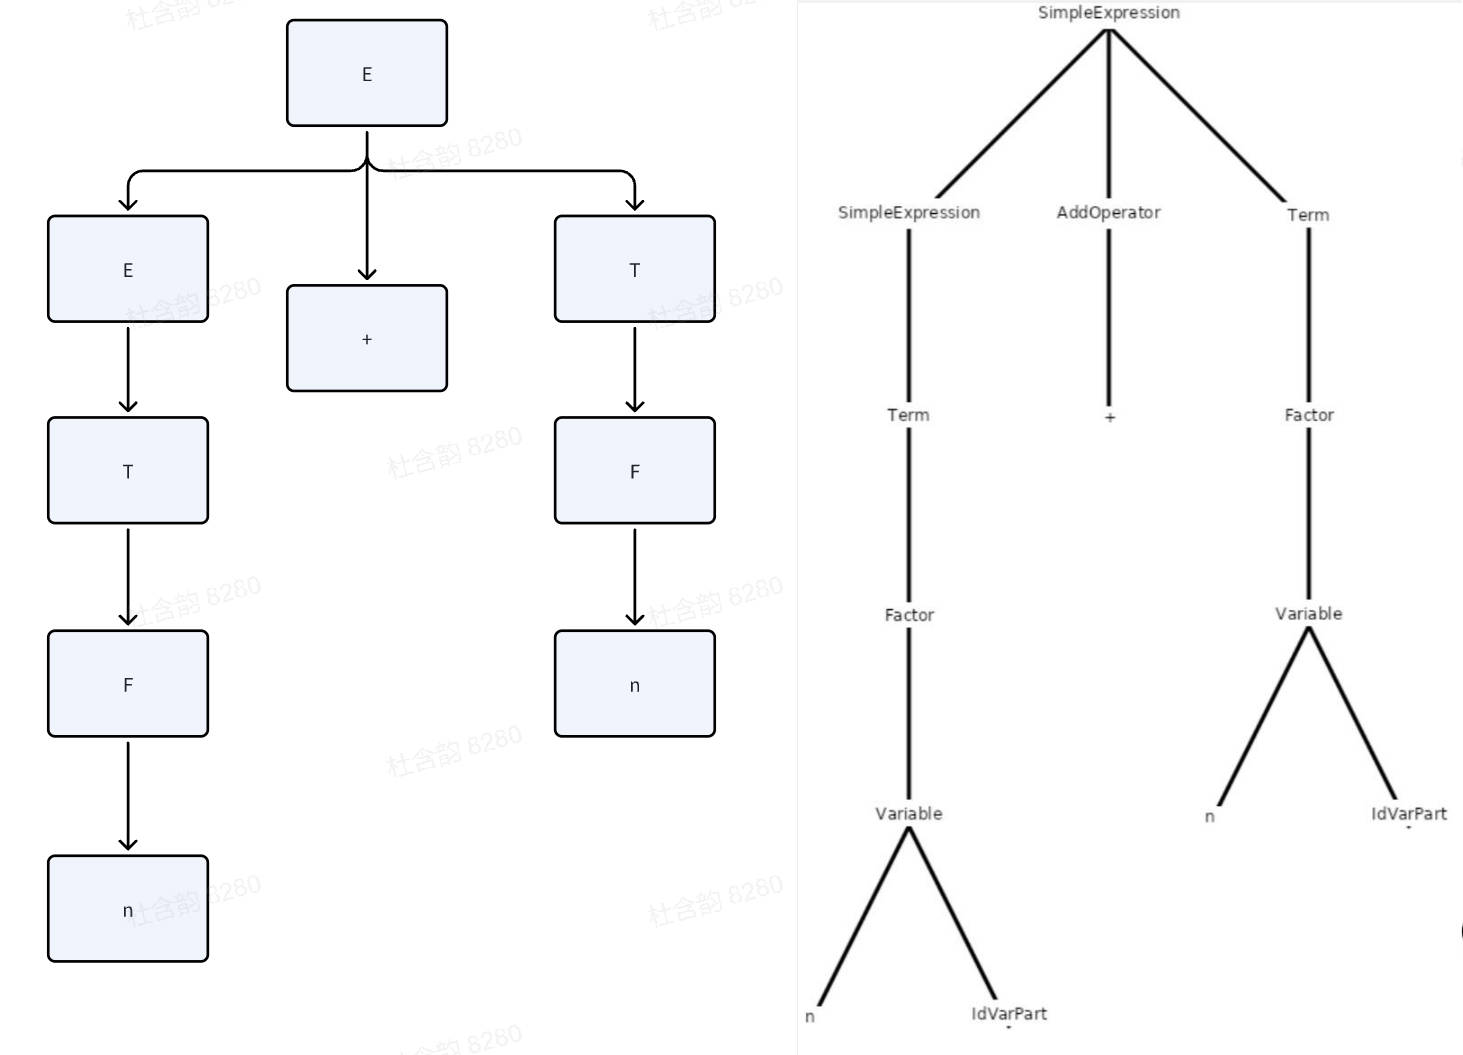
\includegraphics[width=0.8\textwidth]{assets/测试/n+n语法树.jpg}
    \caption{\texttt{n+n}的语法树}
    \label{fig:grammar_1_tree_1}
\end{figure}
\clearpage
使用上述构建的分析表对\texttt{(n+n)*n}句子进行分析。

\begin{figure}[H]
    \centering
    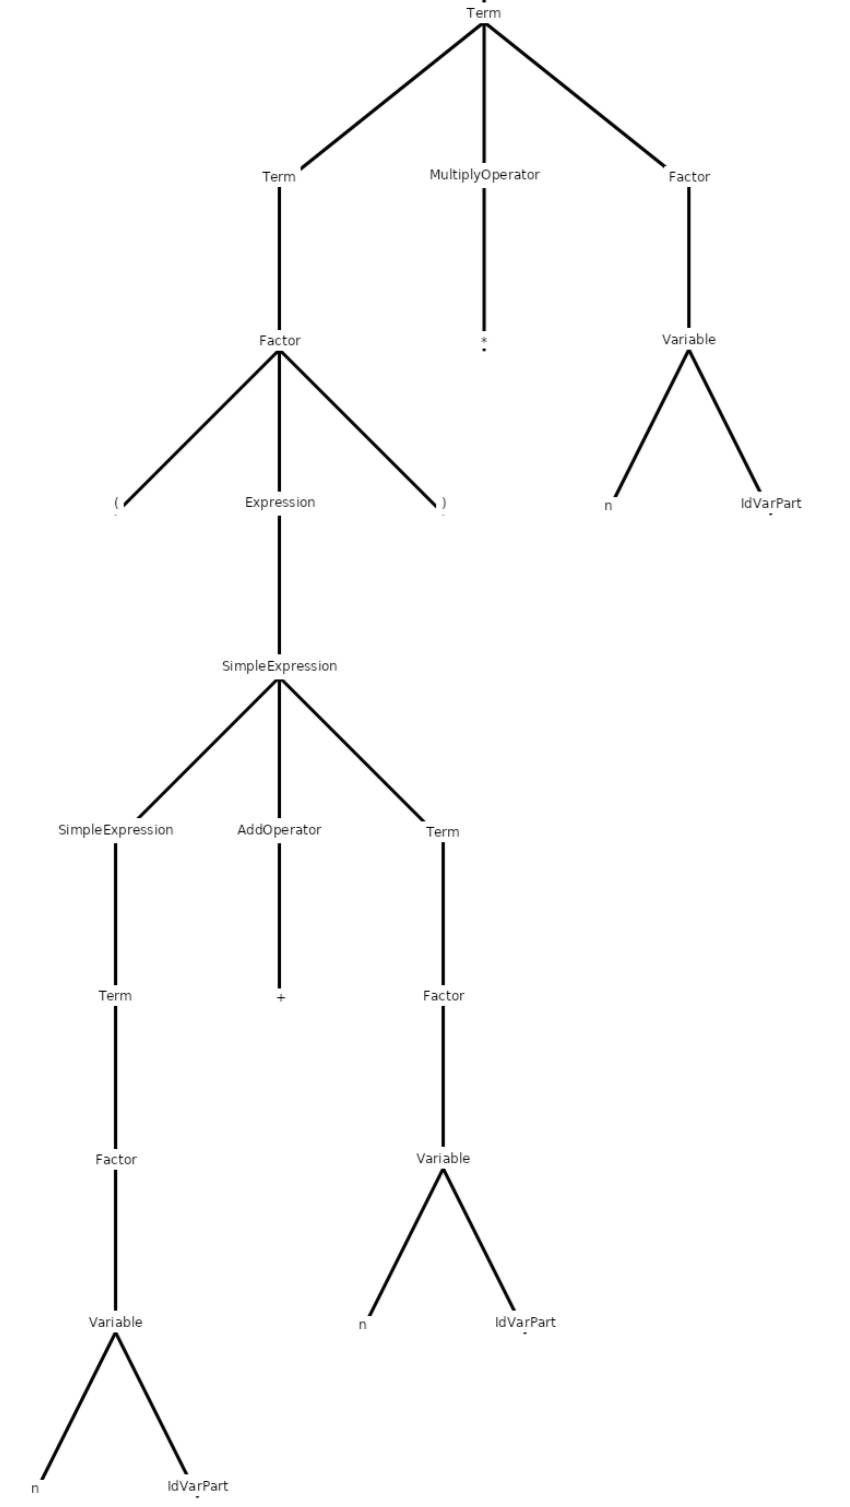
\includegraphics[width=0.7\linewidth]{assets/测试/(n+n)n语法树.jpg}
    \caption{\texttt{(n+n)*n}的语法树}
    \label{fig:grammar_1_tree_2}
\end{figure}


\paragraph{含有空产生式的简单语法测试}

使用含有空产生式的简单语法对构建LR(1)自动机的逻辑进行测试。使用该语法主要测试两个功能:(1) 程序能否正确的处理含有空产生式的语法,包括构建First集合、自动机等部分;(2) 该语法中含有一个移进-归约冲突,使用该语法也可以验证程序是否能够正确识别出该冲突。

\begin{lstlisting}[style=grammar]
Start -> ProgramStruct
ProgramStruct -> ProgramBody ProgramStruct | $\epsilon$ 
ProgramBody -> identifier ProgramBody | identifier
\end{lstlisting}

\texttt{FirstSetTest} 测试程序构建的First集合是否正确,其中手动构建的结果如表\ref{tab:grammar_2_first}所示,测试程序如下所示:

\begin{lstlisting}[style=csharp]
Assert.Contains(builder.FirstSet, pair =>
{
    if (pair.Key == new NonTerminator(NonTerminatorType.StartNonTerminator))
    {
        Assert.Equal(2, pair.Value.Count);
        Assert.Contains(Terminator.IdentifierTerminator, pair.Value);
        Assert.Contains(Terminator.EmptyTerminator, pair.Value);
        return true;
    }

    return false;
});

Assert.Contains(builder.FirstSet, pair =>
{
    if (pair.Key == new NonTerminator(NonTerminatorType.ProgramStruct))
    {
        Assert.Equal(2, pair.Value.Count);
        Assert.Contains(Terminator.IdentifierTerminator, pair.Value);
        Assert.Contains(Terminator.EmptyTerminator, pair.Value);
        return true;
    }

    return true;
});

Assert.Contains(builder.FirstSet, pair =>
{
    if (pair.Key == new NonTerminator(NonTerminatorType.ProgramBody))
    {
        Assert.Single(pair.Value);
        Assert.Contains(Terminator.IdentifierTerminator, pair.Value);
        return true;
    }

    return false;
});
\end{lstlisting}

\begin{table}[h] 
\centering % 让表格内的文字居中
\caption{文法2的First集}
\label{tab:grammar_2_first}
\begin{tabular}{|c|p{10cm}|} % 修改第一列为居中显示
\hline
\textbf{文法符号} & \textbf{First集合} \\ 
\hline
S & a $\epsilon$\\ 
A & a $\epsilon$\\ 
B & a \\ 
\hline
\end{tabular}
\end{table}

\paragraph{正常语法测试}
我们通过以下测试案例验证了编译器对Pascal程序的正确解析能力,并附上相关代码以示例:

\texttt{无操作测试(DoNothingTest)}
\begin{lstlisting}[style=csharp]
const string program = """
                       program DoNothing;
                       begin
                       end.
                       """;
ProgramStruct root = CompilerHelpers.Analyse(program);
Assert.Equal("DoNothing", root.Head.ProgramName.LiteralValue);
Assert.Equal(15, root.Count());
\end{lstlisting}
验证编译器是否能正确解析一个空的Pascal程序。此测试通过,证明编译器可以正确识别和处理无操作的情况。

\texttt{加法测试(AddTest)}
\begin{lstlisting}[style=csharp]
const string program = """
                       program Add;
                       var a : Integer;
                       begin
                       a := 1 + 1
                       end.
                       """;
ProgramStruct root = CompilerHelpers.Analyse(program);
Assert.Equal("Add", root.Head.ProgramName.LiteralValue);
\end{lstlisting}
测试了基本的算术运算,确保编译器可以解析并执行简单的加法表达式。

\texttt{输出测试(WriteLnTest)}
\begin{lstlisting}[style=csharp]
const string program = """
                       program exFunction;
                       const str = 'a';
                       var a, b : Integer;
                       begin
                       writeln( str, ret );
                       end.
                       """;
ProgramStruct root = CompilerHelpers.Analyse(program);
Assert.Equal("exFunction", root.Head.ProgramName.LiteralValue);
\end{lstlisting}
验证了编译器是否能处理包含输出语句的程序。通过正确解析 \texttt{writeln} 语句,测试确认了编译器的I/O语句解析能力。

\texttt{数组和过程测试}
包括了数组声明和使用,以及过程的定义和调用的测试(如 \texttt{ArrayTest}, \texttt{MultiplyArrayTest}, \texttt{ProcedureTest})。这些测试验证了编译器在处理复杂数据结构和程序结构时的准确性。

\texttt{控制流测试}
通过 \texttt{ForLoopTest} 和 \texttt{IfConditionTest} 等测试,检验了编译器对循环和条件判断的处理。确保编译器可以正确解析和执行这些控制流结构。

\paragraph{异常语法测试}
在这一部分,我们测试了编译器在面对不符合语法规则的Pascal代码时的错误处理能力。以下是一些关键的测试案例和对应的代码:

\texttt{结构测试(StructTest)}
\begin{lstlisting}[style=csharp]
const string program = """
                       program main;
                       begin
                       end
                       """;
CatchException(program);
\end{lstlisting}
测试了最基本的程序结构,确认当程序体为空时,编译器是否能正确无返回。此测试通过,说明编译器可以处理空的程序主体。

\texttt{赋值测试(AssignTest)}
\begin{lstlisting}[style=csharp]
const string program = """
                       program main;
                       begin
                        a := 'a';
                       end.
                       """;
CatchException(program);
\end{lstlisting}
尝试在程序中对字符进行赋值,这在Pascal语言中通常是非法的。测试验证了编译器能够抛出并捕获预期的语法错误。

\texttt{语句测试(StatementTest)}
\begin{lstlisting}[style=csharp]
const string program = """
                       program main;
                       begin
                       if a = 1 then
                       doSomething;
                       else
                       doSomething;
                       end.
                       """;
CatchException(program);
\end{lstlisting}
检测了编译器对复杂语句的处理,如条件语句内部缺失正确的语句块界定。此测试确保编译器能识别并报告不完整的条件语句。

\texttt{循环测试(ForTest)}
\begin{lstlisting}[style=csharp]
const string program = """
                       program main;
                       begin
                       for a = 1 to 100 do
                        doSomething
                       end.
                       """;
CatchException(program);
\end{lstlisting}
在此测试中,\texttt{for} 循环缺失了结束分号,编译器需要能识别这一点并生成错误。这证明了编译器在解析循环结构时的准确性。

每个测试都通过引发和捕获 \texttt{GrammarException} 来验证错误处理机制的有效性。

\subsubsection{生成语法分析表测试}

本部分中主要验证内存中的LR(1)分析表和源代码形式的分析表是否一致。

\texttt{ConsistencyTests} 该测试通过遍历内存中的分析表和源代码形式的分析表进行比较,确保其的每一个状态和其迁移到的状态都是一致的。



\subsubsection{语义分析}

语义分析的测试主要包含了类型检查、符号表生成、事件机制触发等方面。

\paragraph{类型检查}
\subparagraph{TypeCheckVisitorTests.cs}
该测试主要通过对不同类型的变量参数进行单独测试以及混合测试来验证类型检查的健壮性。如:常量类型,单个变量类型,多个变量类型,数组类型,过程参数类型,过程中的变量参数类型等。

\begin{itemize}
    \item \textbf{ConstTypeTest}
    \begin{lstlisting}[style=csharp]
const string program = """
      program main;
      const a = 1; b = 1.23; c = 'a';
      begin
      end.
      """;
    \end{lstlisting}

检查常量声明类型是否与符号表中类型一致。

    \item \textbf{SingleTypeTest}
    \begin{lstlisting}[style=csharp]
const string program = """
      program main;
      var a : integer; b : char; c : boolean; d : real;
      begin
      end.
      """;
    \end{lstlisting}

检查变量声明类型是否与是否与符号表中类型一致。

    \item \textbf{MulitpleTypeTest}
    \begin{lstlisting}[style=csharp]
const string program = """
      program main;
      var a, b, c, d : integer;
      e, f, g : boolean;
      begin
      end.
      """;        
    \end{lstlisting}

检查多个同一类型的变量声明是否与符号表中类型一致。

    \item \textbf{ArrayTest}
    \begin{lstlisting}[style=csharp]
const string program = """
      program main;
      var a : array [0..10] of integer;
      b : array [0..10, 0..20] of integer;
      c : array [100..200, 1..5] of real;
      begin
      end.
      """;
    \end{lstlisting}

检查多个数组变量声明是否与符号表中类型一致,包括名字、数组元素类型和数组范围大小。

    \item \textbf{ProcedureParameterTest}
    \begin{lstlisting}[style=csharp]
const string program = """
      program main;
      procedure test(a, b, c : integer);
      begin
      end;
      begin
      end.
      """;        
    \end{lstlisting}

检查过程声明与声明变量是否与符号表中类型一致。

    \item \textbf{ProcedureVarParameterTest}
    \begin{lstlisting}[style=csharp]
const string program = """
      program main;
      procedure test(var a, b, c : real);
      begin
      end;
      begin
      end.
      """;
    \end{lstlisting}

检查过程声明与声明引用变量是否与符号表中类型一致。

    \item \textbf{ProcedureBothParameterTest}
    \begin{lstlisting}[style=csharp]
const string program = """
      program main;
      procedure test(a, b : integer; var c, d: char);
      begin
      end;
      begin
      end.
      """;        
    \end{lstlisting}

检查同时含有引用变量与传值变量的过程声明是否与符号表中类型一致。

    \item \textbf{FunctionBothParameterTest}
    \begin{lstlisting}[style=csharp]
const string program = """
      program main;
      function test(a, b : integer; var c, d: char) : real;
      begin
      end;
      begin
      end.
      """;        
    \end{lstlisting}

检查同时含有引用变量与传值变量的函数声明是否与符号表中类型一致。

    \item \textbf{ProcedureAndFunctionTest}
    \begin{lstlisting}[style=csharp]
const string program = """
      program main;
      procedure test1(a : integer; var b, c : real; d: boolean);
      begin
      end;
      function test2(var a, b : boolean) : boolean;
      begin
      end;
      begin
      end.
      """;
    \end{lstlisting}

检查同时含有引用变量与传值变量的函数与过程声明是否与符号表中类型一致。

    \item \textbf{SubprogramSymbolTableTest}
    \begin{lstlisting}[style=csharp]
const string program = """
      program main;
      const a = 3;
      var b, c : real;
      procedure test(a : boolean);
      var c, d : char;
      begin
      end;
      begin
      end.
      """;
    \end{lstlisting}

检查子过程符号表与父符号表中存储符号的类型是否正确。

    \item \textbf{VarAssignStatementTest}
    \begin{lstlisting}[style=csharp]
const string program = """
      program main;
      var
      a : char;
      b : integer;
      begin
      b := 3;
      a := b;
      end.
      """;
    \end{lstlisting}

检测能否检查变量赋值表达式两侧符号类型是否一致。这个样例应当为False,因为a、b类型不一致。

    \item \textbf{TryConstAssignStatementTest}
    \begin{lstlisting}[style=csharp]
const string program = """
      program main;
      const
      a = 3;
      var
      b : integer;
      begin
      a := 4;
      end.
      """;    
    \end{lstlisting}

检测能否检查检查常量被重新赋值。

    \item \textbf{FunctionAssignStatementTest}
    \begin{lstlisting}[style=csharp]
const string program = """
      program exFunction;
      var
         a, b, ret : integer;
      function max(num1, num2: integer): integer;
      var
           error:char;
         result: integer;
      begin
         if (num1 > num2) then
            result := num1
         else
            result := num2;
         max := error;
      end;
      begin
         a := 100;
         b := 200;
         (* calling a function to get max value *)
         ret := max(a, b);
      end.
      """;  
    \end{lstlisting}

检测能否检查到函数实际返回值与声明函数返回值类型不一致。

    \item \textbf{IfStatementTest}
    \begin{lstlisting}[style=csharp]
const string program = """
      program exFunction;
      var
         a, b, ret : integer;
      begin
         a := 100;
         b := 200;
         if 200 then
             begin
               b := 100;
             end
             else
         b:=200;
      end.
      """;      
    \end{lstlisting}

检测能否检查到if条件表达式类型必须为boolean。

    \item \textbf{ForStatementTest}
    \begin{lstlisting}[style=csharp]
const string program = """
      program exFunction;
      var
         a, b, ret : integer;
         c : char;
      begin
         for a := c to b do
          begin
          b:=b+10;
          end;
      end.
      """;       
    \end{lstlisting}

检测能否检查到for循环语句起始和结束参数类型必须为integer。

    \item \textbf{ProcedureCallTest}
    \begin{lstlisting}[style=csharp]
const string program = """
      program main;
      var
         a, b, c,  min: integer;
         error:char;
      procedure findMin(x, y, z: integer; var m: integer);
      begin
      end;
      begin
         findmin(a, b, c,error);
         (* Procedure call *)
      end.
      """;
    \end{lstlisting}

检测能否检查到调用过程时传参必须与声明时类型一致。

此处还检查了调用函数时传入变量到引用变量的转换是否正确。

    \item \textbf{RecursionProcedureCallTest}
    \begin{lstlisting}[style=csharp]
const string program = """
      program main;
      var a, b:integer; c:real;
      function Test0(var a1:integer; b1:integer; c1:real):integer;
      begin
      test0(a1,b1,c1+0.5);
      end;
      function Test1(var a1:integer; b1:integer; c1:real):integer;
      begin
      test0(1,1,1.0);
      end;
      begin
      teSt1(a,b,1.02);
      test(a, b, c);
      end.
      """;     
    \end{lstlisting}

检测能否检查在函数中调用函数,或进行函数递归的情形。

同时,检测符号是否大小写不敏感。

这个样例将检查到test函数不存在而置为False。

    \item \textbf{ArrayAssignIndexTest}
    \begin{lstlisting}[style=csharp]
const string program = """
      program main;
      var a : array [0..10, 0..10] of integer;
      function test(a, b : integer) : integer;
      begin
          test := 1;
      end;
      begin
      a[0, 1.5] := 1;
      end.
      """;   
    \end{lstlisting}

检测能否检查为数组元素赋值时,下标不为integer的情形。

    \item \textbf{ArrayAssignDimensionTest}
    \begin{lstlisting}[style=csharp]
const string program = """
      program main;
      var a : array [0..10, 0..10] of integer;
      begin
      a[0,1,3] := 1;
      end.
      """;      
    \end{lstlisting}
    
检测能否检查为数组元素赋值时,元素维度错误的情形。

    \item \textbf{ArrayAssignTypeTest}
    \begin{lstlisting}[style=csharp]
const string program = """
      program main;
      var
      a : array [0..10, 0..10] of integer;
      b : array [0..10, 0..20] of integer;
      c : integer;
      d : char;
      begin
      a[0,1] := c;
      c := b[0,5];
      a[0,1] := b;
      end.
      """;
    \end{lstlisting}

检测能否检查为数组元素赋值时,表达式两侧类型不一致的情形。

    \item \textbf{ArrayCalculationTest}
    \begin{lstlisting}[style=csharp]
const string program = """
      program main;
      var a: array[9..12, 3..5, 6..20] of real;
      b: array[0..10] of integer;
      begin
      a[9, 4, 20] := 3.6 + b[5];
      end.
      """;    
    \end{lstlisting}

检测能否检查为数组元素赋值时,表达式右侧为复杂表达式时两侧类型不一致的情形。

同时,还检测了integer与real类型做运算时,integer类型能否被正确转换为real类型。

    \item \textbf{BooleanOperatorTest}
    \begin{lstlisting}[style=csharp]
const string program = """
      program main;
      var flag, tag : boolean;
      error:integer;
      begin
          tag := flag or tag;
          flag := flag and error;
      end.
      """;
    \end{lstlisting}

检测能否检查到变量进行布尔关系运算时,关系符两侧变量不为boolean的情形。

    \item \textbf{TrueFalseTest}
    \begin{lstlisting}[style=csharp]
const string program = """
      program main;
      var a : boolean;
      begin
       a := true;
       a := false;
      end.
      """;
    \end{lstlisting}

检测能否检查到为boolean类型变量赋值时的类型问题。

    \item \textbf{NotTest}
    \begin{lstlisting}[style=csharp]
const string program = """
      program main;
      var a: integer;
      begin
      a := 60;
      write(not a);
      end.
      """;
    \end{lstlisting}
    
检测能否检查到not操作符参与运算时可能出现的问题。

不要求not右侧变量类型一定为boolean,因为not本质是将位取反。

    \item \textbf{PascalFunctionTest}
    \begin{lstlisting}[style=csharp]
const string program = """
      program main;
      var a : integer;
      begin
      write(a);
      read(a);
      writeln(a);
      end.
      """;
    \end{lstlisting}

检查使用函数库的函数能否被正确调用。

    \item \textbf{FunctionCalculateTest}
    \begin{lstlisting}[style=csharp]
const string program = """
      program main;
      var a : integer;
      function test : integer;
      begin
       test := 1;
      end;
      begin
      a := a + test;
      end.
      """;
    \end{lstlisting}

检测能否检查到无参函数返回值在表达式中使用时产生的类型问题。

    \item \textbf{FunctionParameterCalculationTest}
    \begin{lstlisting}[style=csharp]
const string program = """
      program main;
      var a : integer;
      function test (p : integer) : integer;
      begin
      test := p;
      end;
      begin
      a := 1 + test(1);
      end.
      """;
    \end{lstlisting}

检测能否检查到带参函数返回值在表达式中使用时产生的类型问题。
    
\end{itemize}


\paragraph{事件机制触发}

\subparagraph{ConstValueTests.cs}
该测试由事件驱动,检查在访问常量值节点时,能否正确触发事件。

\begin{lstlisting}
    const string program = """
                               program main;
                               const a = 1;
                               begin
                               end.
                               """;
\end{lstlisting}



\paragraph{符号表生成}
\subparagraph{PascalTypeTests.cs}
该测试主要检查了对于复杂类型数组和函数的符号识别与加入符号表的过程正确性。

\begin{lstlisting}[style=csharp]
    [Fact]
    public void PascalArrayTypeTests()
    {
        PascalType array1 = new PascalArrayType(PascalBasicType.Integer, 0, 10);
        PascalType array2 = new PascalArrayType(PascalBasicType.Integer, 0, 10);

        Assert.Equal(array1, array2);
    }

    [Fact]
    public void PascalFunctionTypeTests()
    {
        PascalType function1 = new PascalFunctionType([new PascalParameterType(PascalBasicType.Integer, false, "a")],
            PascalBasicType.Void);
        PascalType function2 = new PascalFunctionType([new PascalParameterType(PascalBasicType.Integer, false, "a")],
            PascalBasicType.Void);

        Assert.Equal(function1, function2);
    }
\end{lstlisting}

\subparagraph{SymbolTableTests.cs}
该测试检查了符号表能否正确获取基本类型,能否正确插入和查找符号。对于作用域规则,在符号表存在嵌套情况时,向子符号表插入符号能否在子符号表和父符号表中查找来验证符号表的生成。

\begin{lstlisting}[style =csharp]
    [Fact]
    public void NestedTableInsertAndFindTest()
    {
        SymbolTable table = new();

        Assert.True(table.TryAddSymbol(new Symbol { SymbolName = "a", SymbolType = PascalBasicType.Integer }));
        Assert.True(table.TryAddSymbol(new Symbol
        {
            SymbolName = "temperature", SymbolType = PascalBasicType.Real, Const = true
        }));

        SymbolTable child = table.CreateChildTable();

        Assert.True(child.TryAddSymbol(new 
    }
\end{lstlisting}

\paragraph{与其他部分的协同合作}

\subparagraph{SyntaxTreeTravellerTests.cs}
该测试实现的是语义分析和语法分析的协同,对于已经创建好的语法树,语义分析能否正确工作。测试通过遍历语法树并得到正确结果验证了语义分析的协同功能。

\begin{lstlisting}[style =csharp]
const string program = """
      program main;
      begin
      end.
      """;

        SampleSyntaxTreeVisitor visitor = new();
        IEnumerable<SemanticToken> tokens = _lexer.Tokenize(new StringSourceReader(program));
        ProgramStruct root = _grammarParser.Analyse(tokens);

        _traveller.Travel(root, visitor);

        List<string> result =
        [
            "ProgramStruct",
            "ProgramHead",
            "ProgramHead",
            "ProgramBody",
            "SubprogramDeclarations",
            "SubprogramDeclarations",
            "CompoundStatement",
            "StatementList",
            "Statement",
            "Statement",
            "StatementList",
            "CompoundStatement",
            "ProgramBody",
            "ProgramStruct"
        ];

        string[] actual = visitor.ToString().Split('\n');

        foreach ((string line, uint index) in result.WithIndex())
        {
            Assert.Equal(line, actual[(int)index]);
        }
    }
\end{lstlisting}

\subsection{集成测试}

集成测试主要针对编译器的完整功能进行测试。而对完成功能进行测试最好的方式即为对比标准Pascal编译器和自行实现的编译器所编译的可执行程序运行结果的差异。因此我们编写了一个简单的Python自动化这个过程:针对输入的Pascal源程序文件和可选的程序输入,分别使用Free Pascal Compiler编译得到可执行程序、再使用自行实现的编译器和GCC编译器进行编译得到可执行程序,分别执行两个可执行程序并比对两个程序输出的结果。

集成测试的运行结果如图\ref{fig:integrated_test_figure}所示:

\begin{figure}
    \centering
    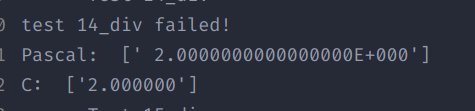
\includegraphics[width=0.5\linewidth]{assets/集成测试示例.png}
    \caption{集成测试的示例}
    \label{fig:integrated_test_figure}
\end{figure}

同时需要指出的是,我们在实践的过程中发现自行搭建的集成测试运行结果和头歌平台运行的结果不同,列举如下:
\begin{itemize}
    \item 对于\texttt{real}类型数据的输出格式不同。在自行搭建的平台上输出的格式为空格+科学记数法格式,而在头歌平台上则是没有空格和保留6位小数的格式。
    \item 部分测试点存在头歌上的运行结果和本地运行的结果不同的问题。
\end{itemize}

\subsection{持续测试}

在多人协作进行项目开发时,如何确保每个人编写的代码能够正常工作并且不会破坏程序其他部分的运行是一个重要的问题。因此,在本次的程序开发过程中,我们基于\href{https://gitea.com}{Gitea}提供了丰富CI/CD功能提供在每个提交新的代码和将代码合并到主线时自动运行所有的单元测试和集成测试的功能。

\begin{figure}[htbp]
    \centering
    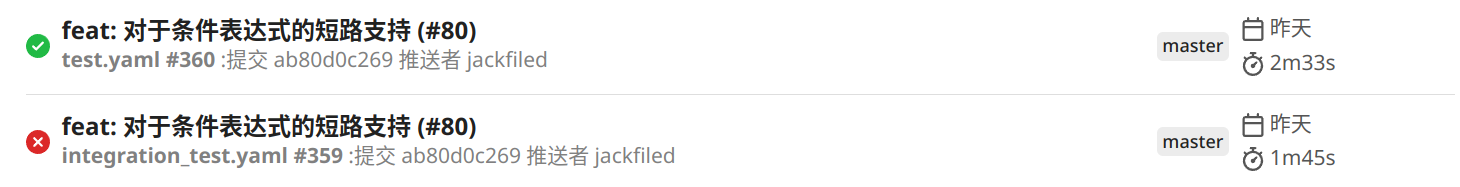
\includegraphics[width=0.8\linewidth]{assets/持续测试示例.png}
    \caption{持续测试的运行示例}
    \label{fig:continous_test_example}
\end{figure}

\end{document}
